\documentclass[11pt]{article}
\usepackage[latin1]{inputenc}
\usepackage{a4wide}
\usepackage{amsmath}
\usepackage{amsfonts}
\usepackage{amssymb}
\usepackage{graphicx}
\usepackage{enumerate}
\usepackage{epstopdf}
\usepackage{float}
\usepackage{multicol}
\usepackage{hyperref}
\epstopdfsetup{outdir=./images/}
\usepackage{subcaption}

\title{Natural Computing, Assignment 3}
\author{Dennis Verheijden - s4455770 \and Pauline Lauron - s1016609 \and Joost Besseling - s4796799}
\begin{document}
\maketitle

\section{}
\begin{enumerate}[(a)]
\item Updating is done by:
\begin{align}
x(i;d)^{t+1} &= x(i,d)^t + v(i;d) \\
x(i)^{t+1} &= (x(i,0)^t + v(i,0), \quad x(i,1)^t + v(i,1)) 
\end{align}
So the next position of the particles after one iteration of the PSO algorithm with $w=2, r_1 = r_2 = 0.5$ are:
\begin{align*}
v(1,0) &= 2 \times 2 + 0.5 \times (5 - 5) + 0.5 \times (5 - 5) = 4 \\
v(1,1) &= 2 \times 2 + 0.5 \times (5 - 5) + 0.5 \times (5 - 5) = 4 \\
x(1)^1 &= (5 + 4, \quad 5 + 4) = (9, 9) \\ \\6
x(2)^1 &= (8 + (2 \times 3 + 0.5 \times (7 - 8) + 0.5 \times (5 - 8)), \\
 &\qquad   3 + (2 \times 3 + 0.5 \times (3 - 3) + 0.5 \times (5 - 3))) \\
       &= (8 + 4, \quad 3 + 7) = (12, 10) \\ \\
x(3)^1 &= (6 + (2 \times 4 + 0.5 \times (5 - 6) + 0.5 \times (5 - 6)), \\
 &\qquad   7 + (2 \times 4 + 0.5 \times (6 - 7) + 0.5 \times (5 - 7))) \\
       &= (6 + 7, \quad 7 + 6.5) = (13, 13.5)
\end{align*}

\item The next position of the particles after one iteration of the PSO algorithm with $w=0.1, r_1 = r_2 = 0.5$ are:
\begin{align*}
x(1)^1 &= (5 + (0.1 \times 2 + 0.5 \times (5 - 5) + 0.5 \times (5 - 5)), \\
 &\qquad   3 + (0.1 \times 2 + 0.5 \times (5 - 5) + 0.5 \times (5 - 5))) \\
       &= (5 + 0.2, \quad 5 + 0.2) = (5.2, 5.2) \\ \\
x(2)^1 &= (8 + (0.1 \times 3 + 0.5 \times (7 - 8) + 0.5 \times (5 - 8)), \\
 &\qquad   3 + (0.1 \times 3 + 0.5 \times (3 - 3) + 0.5 \times (5 - 3))) \\
       &= (8 - 1.7, \quad 3 + 1.3) = (6.3, 4.3) \\ \\
x(3)^1 &= (6 + (0.1 \times 4 + 0.5 \times (5 - 6) + 0.5 \times (5 - 6)), \\
 &\qquad   7 + (0.1 \times 4 + 0.5 \times (6 - 7) + 0.5 \times (5 - 7))) \\
       &= (6 - 0.6 , \quad 7 - 1.1) = (5.4, 5.9)
\end{align*}

\item The effect of $w$ is the importance of the velocity of the particle for updating. Setting this value lower (in proportion to $r_1$ and $r_2$) decreases the effect of the particle and increases the effect of the particle best and the social best. This effectively makes the particle more inclined to move towards the social and its personal best.

\item The advantage of a high value of $w$ is that the impact of individual particles is larger, such that they maintain the same velocity and direction. The disadvantage is that the effect of the swarm becomes less significant.
\end{enumerate}


\section{}
% NOTE: MIGHT BE WRONG, MORE THINKING NEEDED
If the swarm would only consist of a single member and $w < 1$, it wouldn't perform very well. 

Say the initial velocity and position are positive. Then the personal influence would be zero (personal best would equal current position) and the social influence would also be zero (the particle is the population). The initial iteration would thus result in a positive update, moving away from the global and local optima. 

After the first iteration, assuming $r_1 > w$, there will be a negative update, since the personal influence becomes negative and is bigger than the inertia influence.

This would iterate for a very long time, but we think because of the last negative update, we would eventually reach (or get close to) the optimal value. This is assuming we don't draw random numbers for $r_1$.

\section{}
For this exercise we implemented PSO and compared it to Kmeans. Both are implementations as proposed in the supplied paper.As PSO relies on randomness (apart from instantiation) by the two random parameters $r_1$ and $r_2$, we run the PSO algorithm 10 times. The results may be found in figure \ref{fig:pso_kmeans}. 

Here we can see that there is quite some variation for the results of PSO. We also see that every run converges, in the sense that the algorithm cannot find a better result at some point in time. The algorithm itself however, does not converge in any run as was evident from the output.

Another thing, which is probably the most obvious, is that PSO never manages to beat kmeans in terms of quantization error. However our implementation does not manage to get the results that were reported in the paper, so there could be a mistake in the code. We do use the \textit{best} values for $w = 0.72$ and $c_1 = c_2 = 1.49$.

\begin{figure}[H]
	\centering
	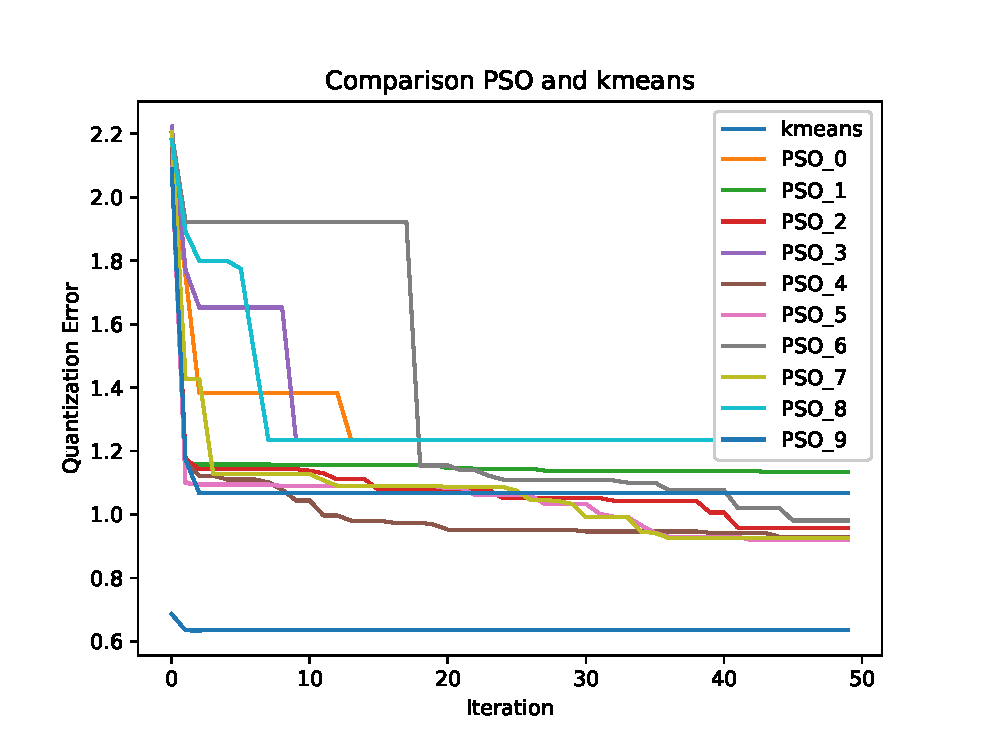
\includegraphics[width=0.7\textwidth]{images/pso_kmeans.eps}
	\caption{Comparison of 10 runs of PSO and kmeans. The quantization error is plotted as a function of iterations.}
	\label{fig:pso_kmeans}
\end{figure}

\section{}

The Tabu list  would prevent the ants from getting stuck in a loop in the bottom part of the image. There are a lot of possibilities for loops here. At many of the decision points in the bottom part, the ant will get a 50-50 or worse choice between going forward or going backward. So a lot of the routes on the bottom will be relatively long.

Only an ant that randomly decides to choose the upper route, would be forced to walk to the end. This would then be the best solution that is found. 

A result of this is that the convergence (if any) is much slower when there is no tabu list versus if such a list is used.

\section{}
Encouraging exploitation means following the pheromone. On the other hand, exploration is encouraged by explicitly not following the pheromone. We can use this and, the fact that the ant is allowed to lay pheromone at every time step to encourage exploration even for ants following the pheromone. Every ant has a chance $p$ to follow the pheromone, and a chance $1 - p$ to go in a random direction. 

If the ant chooses to leave the pheromone path, it lays a certain amount $a$ of pheromone, encouraging other ants to diverge from the path and explore a new route. This greatly increases the chance that one of the exploring ants finds a better route.

Then, if one of the ants finds a better solution, we can put some amount of pheromone proportional to the fitness on the new route.

It might be beneficial to keep track of the difference between the two different types of pheromone, because we don't want the ants to accidentally introduce bad routes, because too many ants follow the 'local' pheromone.

We can increase $p$ over time, to encourage convergence on a single route. 


\section{}


We have implemented the ACO to solve sudoku's in the following way. We let each ant hold the unsolved sudoku, and give it access to the global pheromone matrix. Each ant constructs a solution, based on the pheromone matrix. First, it picks a random unfilled part of the sudoku, then it looks at all unused numbers of the current row and picks one of those numbers according to the pheromone.

The pheromone is represented in the following way: it is a $9\times9\times9$ matrix $P$, where $P[i][j]$ is a list of probabilities. These probabilities denote the chance of each number in $1-9$ being at that $i,j$ in the sudoku.

We initialize the pheromone matrix such that each number has an equal probability of being used. So we fill the matrix with the value $1/9$. After that we let all the ants build their solution. We then pick the best solution, which we define as the solution with the least amount of double numbers per column and per grid. 

We update the pheromone matrix by increasing the probability that the numbers chosen by the best ant, are chosen again. So if the best ant had a 9 on position $(3,3)$, we update $P$ as follows:

\begin{align*}
	P&[i][j][9-1] += p, \\
\end{align*}

where $p$ denotes the amount of added pheromone. Then we normalize the list, to make sure it is a probability vector.

We iterate this process with $n$ ants, for $it$ iterations.

Because we view the pheromone matrix as a matrix of probability vectors, the old pheromone fades because every time we increase the probability of one number, all other probabilities go down. In this way the old pheromone slowly fades away.
 
\ \ \  \ \ \ 






---------------

The fitness is the inverse of the number of collisions (where a collision means that two of the same numbers appear in the same row, column or matrix)

The rows each hold permutations of the 9 numbers. 

The columns and the matrices contribute to the fitness.

The matrix is a stack on top of the sudoku, with for each value, the chance that is should be in that specific spot.

(so layer [1] is the 9x9 matrix that denotes the probabilities of the places where the 1's should go. Layer [9] does the same, but for 9's.)

We construct some solutions based on the matrices, and then update the pheromones, by increasing the chance that the best solution occurs. Alll other values fade some amount.

????



\end{document}